\documentclass{article}
\usepackage{tikz}
\usepackage{amsmath}

\begin{document}

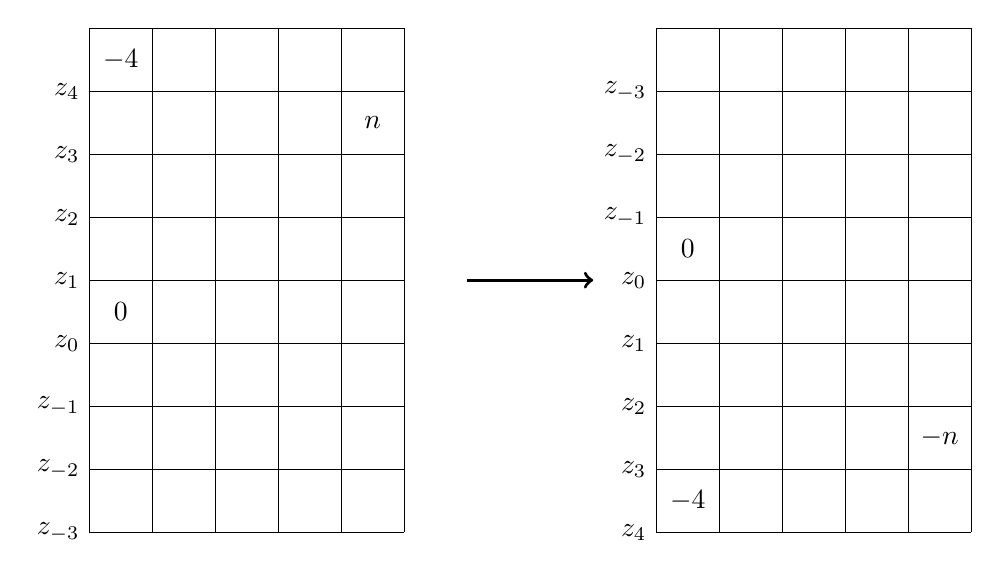
\begin{tikzpicture}[scale=0.8]
% Left grid
\draw (0,0) grid (5,8);

% Labels for left grid
\node[left] at (0,7) {$z_4$};
\node[left] at (0,6) {$z_3$};
\node[left] at (0,5) {$z_2$};
\node[left] at (0,4) {$z_1$};
\node[left] at (0,3) {$z_0$};
\node[left] at (0,2) {$z_{-1}$};
\node[left] at (0,1) {$z_{-2}$};
\node[left] at (0,0) {$z_{-3}$};

\node at (0.5,7.5) {$-4$};
\node at (0.5,3.5) {$0$};

\node at (4.5,6.5) {$n$};

% Arrow
\draw[->, very thick] (6,4) -- (8,4);

% Right grid
\draw (9,0) grid (14,8);

% Labels for right grid
\node[left] at (9,0) {$z_4$};
\node[left] at (9,1) {$z_3$};
\node[left] at (9,2) {$z_2$};
\node[left] at (9,3) {$z_1$};
\node[left] at (9,4) {$z_0$};
\node[left] at (9,5) {$z_{-1}$};
\node[left] at (9,6) {$z_{-2}$};
\node[left] at (9,7) {$z_{-3}$};

\node at (9.5,0.5) {$-4$};
\node at (9.5,4.5) {$0$};

\node at (13.5,1.5) {$-n$};

\end{tikzpicture}

\end{document}